\documentclass[11pt, dvipdfmx]{beamer}
%\documentclass[8,9,10,11,12,14,17,20pt, dvips, handout]{beamer}
%%%%%%%%%%%  package  %%%%%%%%%%%
\usepackage{amssymb,amsmath,ascmac}
\usepackage{atbegshi}
%\usepackage[orientation=portrait, size=a4, debug]{beamerposter}


\AtBeginShipoutFirst{\special{pdf:tounicode 90ms-RKSJ-UCS2}}
\usepackage{minijs}
\renewcommand{\kanjifamilydefault}{\gtdefault}
\usepackage{multirow}
\usepackage{bm}
%\usepackage[dvipdfmx]{graphicx}
%\usepackage{multimedia}

\usepackage{tikz}
\usepackage{xparse}
\usetikzlibrary{shapes,arrows}
%% define fancy arrow. \tikzfancyarrow[<option>]{<text>}. ex: \tikzfancyarrow[fill=red!5]{hoge}
  \tikzset{arrowstyle/.style n args={2}{inner ysep=0.1ex, inner xsep=0.5em, minimum height=2em, draw=#2, fill=black!20, font=\sffamily\bfseries, single arrow, single arrow head extend=0.4em, #1,}}
  \NewDocumentCommand{\tikzfancyarrow}{O{fill=black!20} O{none}  m}{
    \tikz[baseline=-0.5ex]\node [arrowstyle={#1}{#2}] {#3 \mathstrut};}

%微分関連のマクロ
%
\newcommand{\diff}{\mathrm d}
\newcommand{\difd}[2]{\dfrac{\diff #1}{\diff #2}}
\newcommand{\difp}[2]{\dfrac{\partial #1}{\partial #2}}
\newcommand{\difdd}[2]{\dfrac{\diff^2 #1}{\diff #2^2}}
\newcommand{\difpp}[2]{\dfrac{\partial^2 #1}{\partial #2^2}}

%%%%%%%%%%%  theme  %%%%%%%%%%%

%%%%%
% Simple
%%%%%
%\usetheme{default}
%\usetheme{Pittsburgh}
%\usetheme{Rochester}
%\usetheme{Szeged}

%%%%%
% So So
%%%%%
%\usetheme{Singapore}
%\usetheme{CambridgeUS}
\usetheme{Copenhagen}
%\usetheme{Luebeck}
%\usetheme{Malmoe}
%\usetheme{Warsaw}

%%%%%
% No Heasder
%%%%%
%\usetheme{Madrid}
%\usetheme{Boadilla}

%%%%%
% No Footer
%%%%%
%\usetheme{Darmstadt}
%\usetheme{JuanLesPins}
%\usetheme{Montpellier}

%%%%%
% Color
%%%%%
%\usetheme{AnnArbor}

%%%%%
% Too much
%%%%%
%\usetheme{Berlin}
%\usetheme{Ilmenau}

%%%%%
% Right hand Side
%%%%%
%\usetheme{Goettingen}
%\usetheme{Marburg}

%%%%%
% Left hand Side
%%%%%
%\usetheme{PaloAlto}


%%%%%%%%%%%  inner theme  %%%%%%%%%%%
\useinnertheme{default}
%\useinnertheme{circles}
%\useinnertheme{inmargin}
%\useinnertheme{rectangles}
%\useinnertheme{rounded}


%%%%%%%%%%%  outer theme  %%%%%%%%%%%
\useoutertheme{default}
%\useoutertheme{miniframes}
%\useoutertheme{infolines}
%\useoutertheme{miniframes}
%\useoutertheme{smoothbars}
%\useoutertheme{sidebars}
%\useoutertheme{split}
%\useoutertheme{shadow}
%\useoutertheme{tree}
%\useoutertheme{smoothtree}


%%%%%%%%%%%  color theme  %%%%%%%%%%%
%\usecolortheme{structure}
%\usecolortheme{sidebartab}
%\usecolortheme{albatross}
%\usecolortheme{beetle}
%\usecolortheme{dove}
%\usecolortheme{crane}
%\usecolortheme{fly}
%\usecolortheme{seagull}
%\usecolortheme{wolverine}
%\usecolortheme{beaver}
%\usecolortheme{lily}
%\usecolortheme{orchid}
%\usecolortheme{rose}
%\usecolortheme{whale}
%\usecolortheme{seahorse}
%\usecolortheme{dolphin}


%%%%%%%%%%%  font theme  %%%%%%%%%%%
\usefonttheme{professionalfonts}
%\usefonttheme{default}
%\usefonttheme{serif}
%\usefonttheme{structurebold}
%\usefonttheme{structureserif}
%\usefonttheme{structuresmallcapsserif}


%%%%%%%%%%%  degree of transparency  %%%%%%%%%%%
%\setbeamercovered{transparent=30}

%\setbeamercolor{item}{fg=red}
\setbeamertemplate{items}[default]

%%%%%%%%%%%  numbering  %%%%%%%%%%%
%\setbeamertemplate{numbered}

\setbeamertemplate{navigation symbols}{}

\title
{ゴムの破壊\\Andrews 理論}
\author{佐々木裕}
\institute[東亞合成]{東亞合成}
\date{\today}

\begin{document}

%%%%%%%%%%%%%%%%%%%%%%%%%%%%%%%
\begin{frame}\frametitle{}
	\titlepage
\end{frame}



%%%%%%%%%%%%%%%%%%%%
\section{ゴムの破壊}


\subsection{破壊工学の考え方}

%%%%%%%%%%%%%%%%%%%%%%%%%%%%%%%%%%%%%%%
\begin{frame}
\frametitle{破壊工学の考え方}
\begin{exampleblock}{破壊工学の考え方}

\begin{itemize}
\item
系中にクラックが存在することを前提に材料の耐久性を評価
\item
\alert{「クラック近傍での応力集中を如何に抑制するか」}がポイント
\end{itemize}
\end{exampleblock}

\begin{columns}[totalwidth=1\textwidth]
\column{.5\textwidth}
\begin{alertblock}{破壊工学の観点から(微視的)}
	\begin{itemize}
		\item
		クラック先端での応力集中\\ \alert{応力拡大係数 $K_I$ で評価}
		\footnotesize
		\begin{align*}
		K_{I} = \sigma \sqrt{\pi c}
		\end{align*}
		\normalsize
		\item 
		クラック進展の抑制 \\
		$\Rightarrow$ 先端での\alert{局所降伏}\\
		降伏応力 $\sigma_Y$ に反比例
		\footnotesize
		\begin{align*}
		d \propto \left( \dfrac{K_I}{\sigma_Y} \right)^2
		\end{align*}
		\normalsize
	\end{itemize}
\end{alertblock}
\column{.5\textwidth}
	\centering
	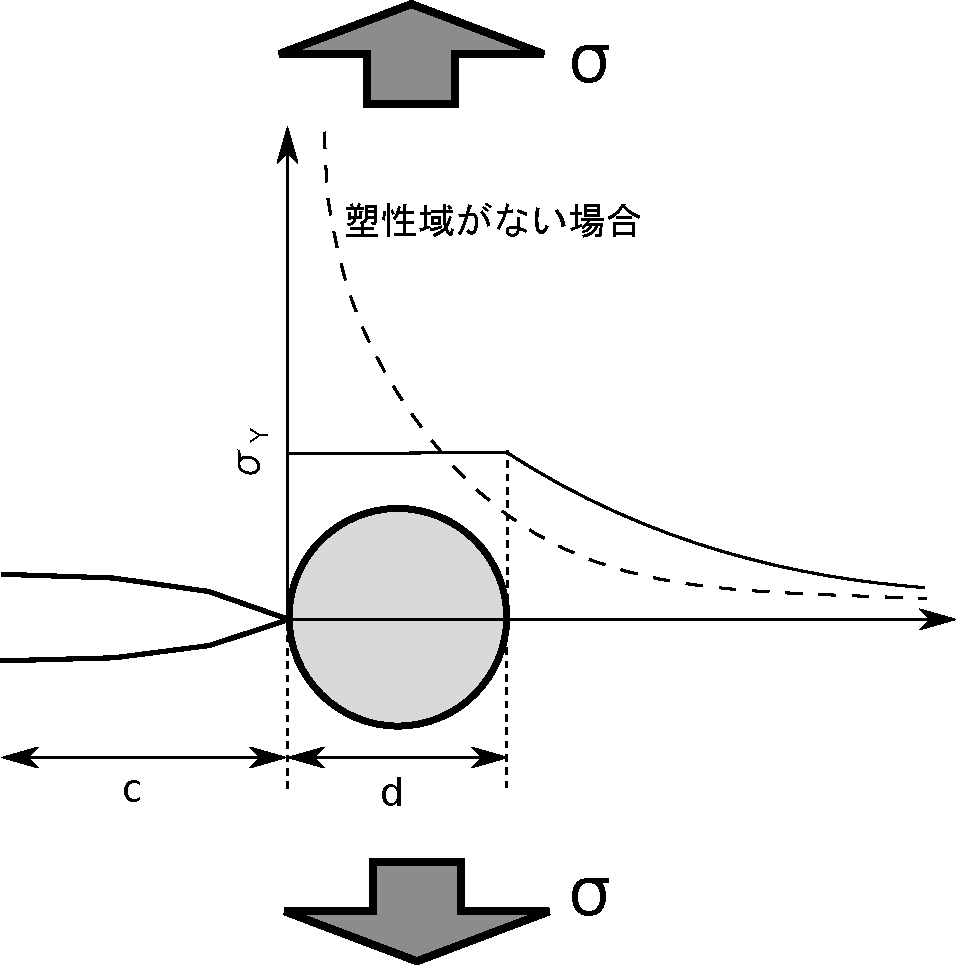
\includegraphics[width=45mm]{fig/Crack_Yield.pdf}
\end{columns}

\end{frame}


\subsection{ゴムの大変形}


%%%%%%%%%%%%%%%%%
\begin{frame}
%[shrink squeeze]
\frametitle{ゴムの亀裂先端近傍での大変形}



\centering
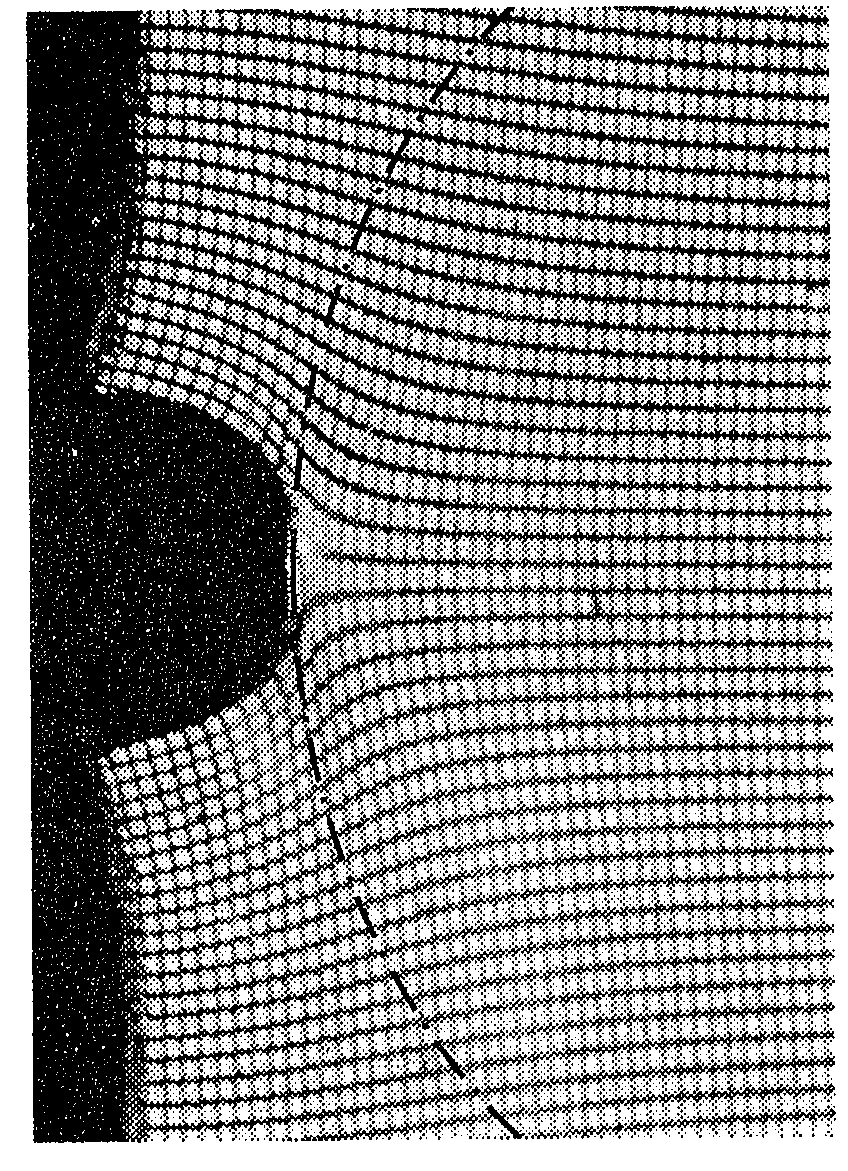
\includegraphics[width=.5\textwidth]{fig/rubber_crack.png}

\end{frame}


\subsection{引き裂きエネルギーの時間温度依存}

%%%%%%%%%%%%%%%%%
\begin{frame}
%[shrink squeeze]
\frametitle{引き裂きエネルギーの時間温度依存}

%\begin{alertblock}{時間温度換算則で考えてみれば?}
%NR の適正な変形速度・温度と SBR のそれとの違い
%\end{alertblock}
%

\begin{columns}[totalwidth=1\textwidth]
\column{.48\textwidth}

粘弾性効果の極限

高温・低速

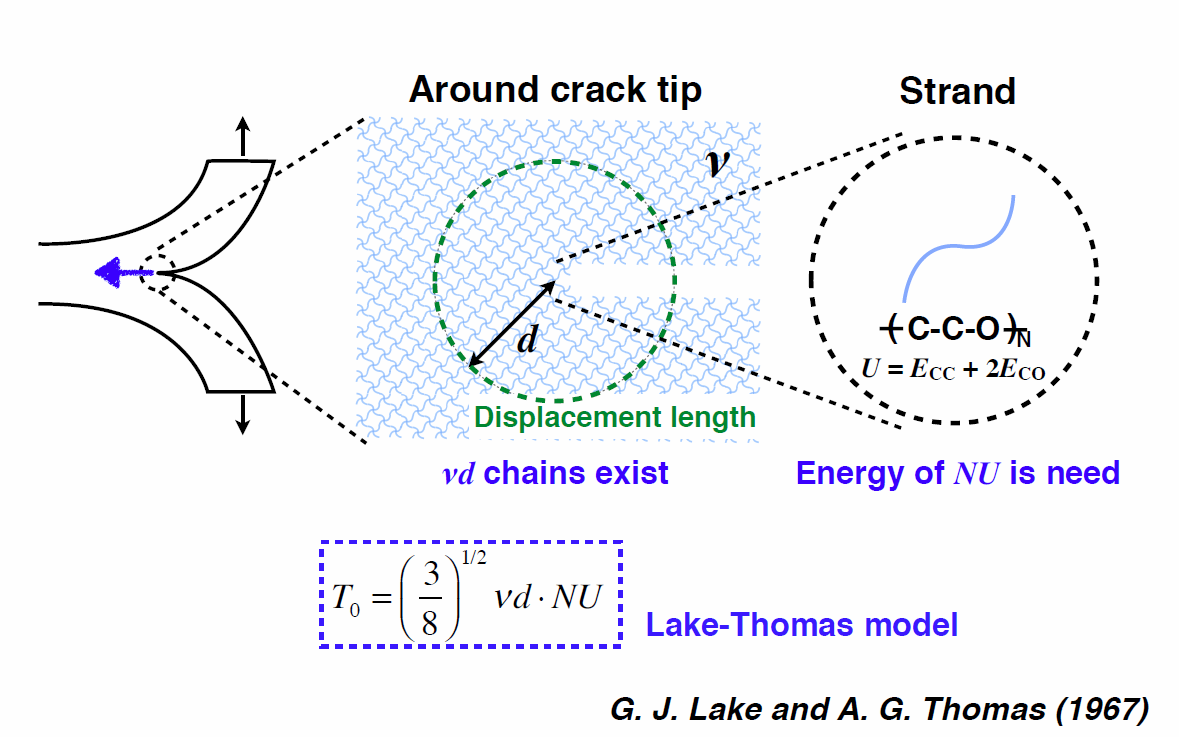
\includegraphics[width=\textwidth]{fig/Lake_Thomas.png}

\column{.48\textwidth}

変形速度、温度に依存

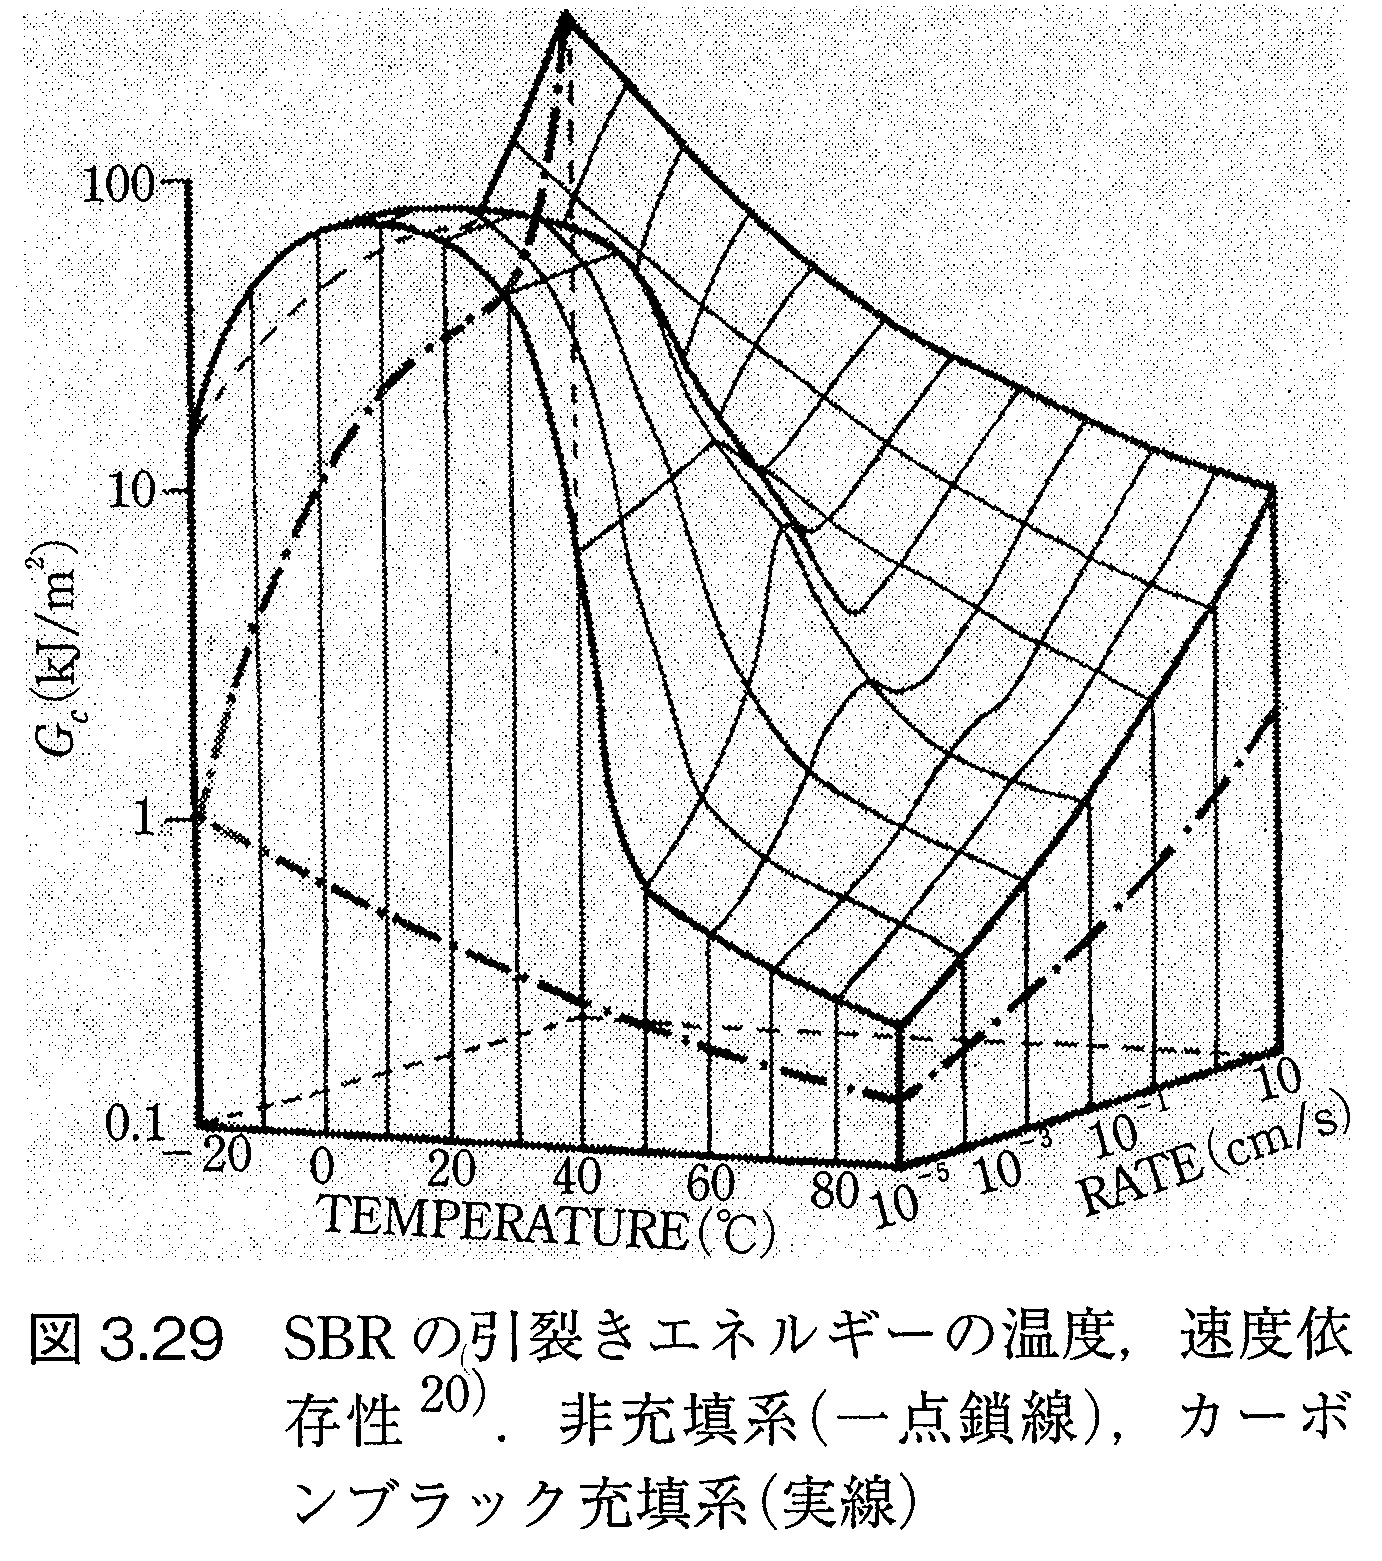
\includegraphics[width=0.8\textwidth]{fig/break_TT.png}

\end{columns}

\begin{alertblock}{ゴムの引き裂きエネルギー}
$\mathcal{T}=\mathcal{T}_0 \Phi(\dot{c}, T, \epsilon_0)$
\end{alertblock}

\end{frame}

%%%%%%%%%%%%%%%%%%%%
\section{理論的アプローチ}



%%%%%%%%%%%%%%%%%%%%%%%%%%%%%
\subsection{Andrews 理論}
%
%%%%%%%%%%%%%%%%%
\begin{frame}
\frametitle{Andrews 理論}

\small

\begin{columns}[totalwidth=1\textwidth]
\column{.6\textwidth}
\begin{exampleblock}{\Large Andrews 理論}
%クラック成長時の応力場の考察より
	\begin{itemize}
	\item
	降伏、ヒステリシスを示す材料では、
		\begin{itemize}
		\item
		Loading 場とUnloading 場が存在
		\item
		この差が、全体の変形に要したエネルギーの多くを散逸
		\end{itemize}	
	\item
	\alert{鎖の破断に使われるエネルギーが低減} \\$\Rightarrow$ 強靭さの起源。
	\item
	実験的に、$\Phi$ を求めている。
	\end{itemize}
\end{exampleblock}

{Andrews, E. H. and Fukahori, Y., Journal of Materials Science, 12, 1307 (1977)}

\column{.4\textwidth}
\centering
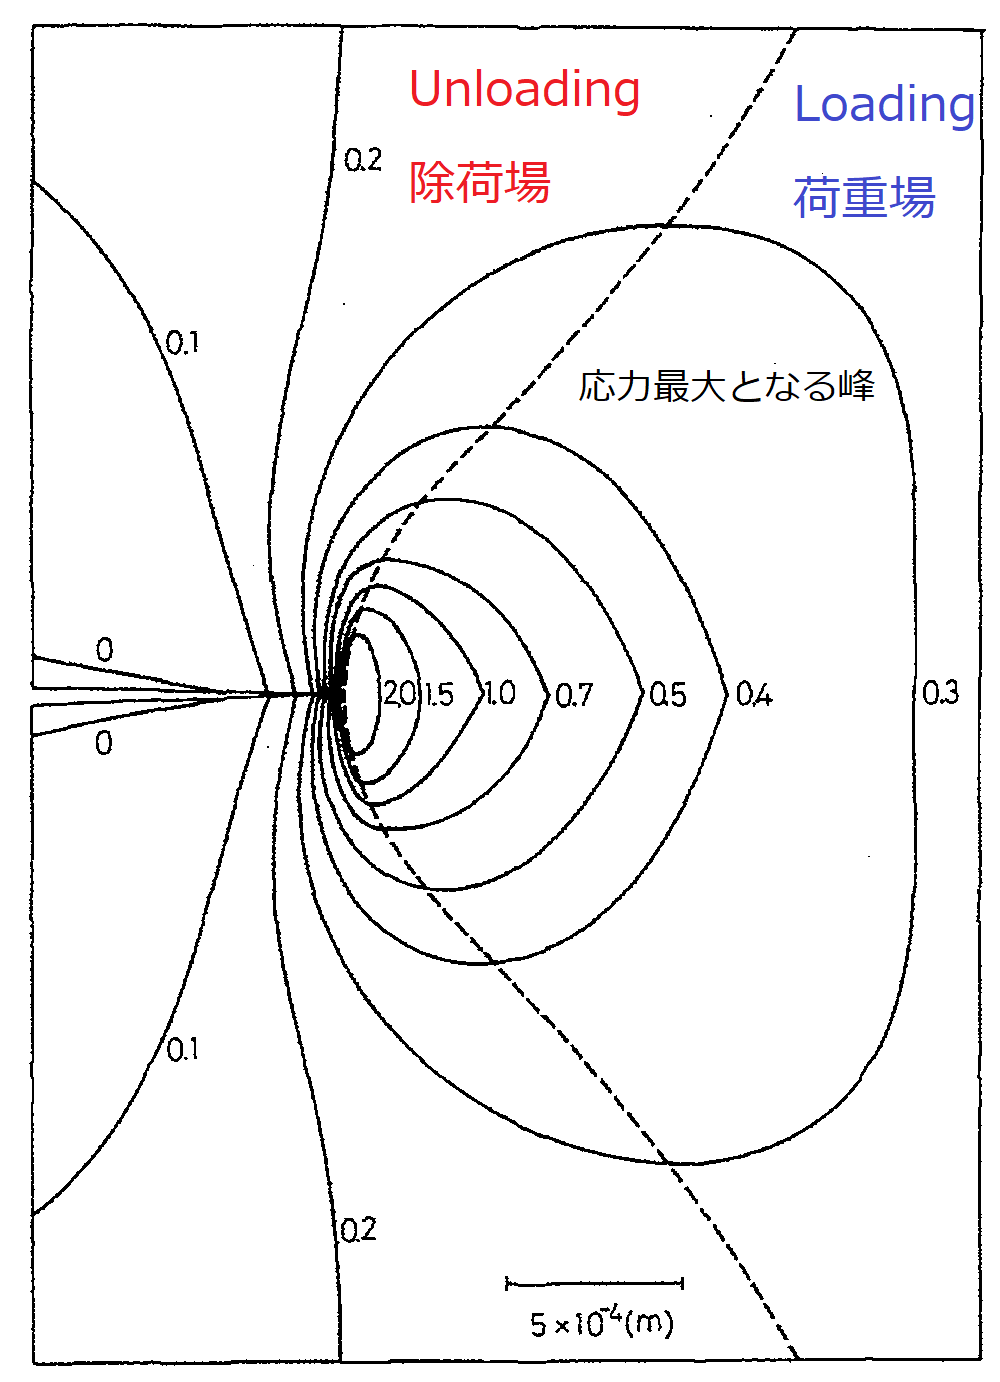
\includegraphics[width=40mm]{fig/crack.png}
\end{columns}

\begin{alertblock}{クラック先端での力学的ヒステリシス}
ミクロな緩和現象がマクロな耐久性向上と繋がる。
\end{alertblock}

\end{frame}

%%%%%%%%%%%%%%%%%%%%%%%%%%%%%%%%
\begin{frame}
\frametitle{補足}

\begin{columns}[T, totalwidth=0.96\linewidth]
\column{.47\linewidth}

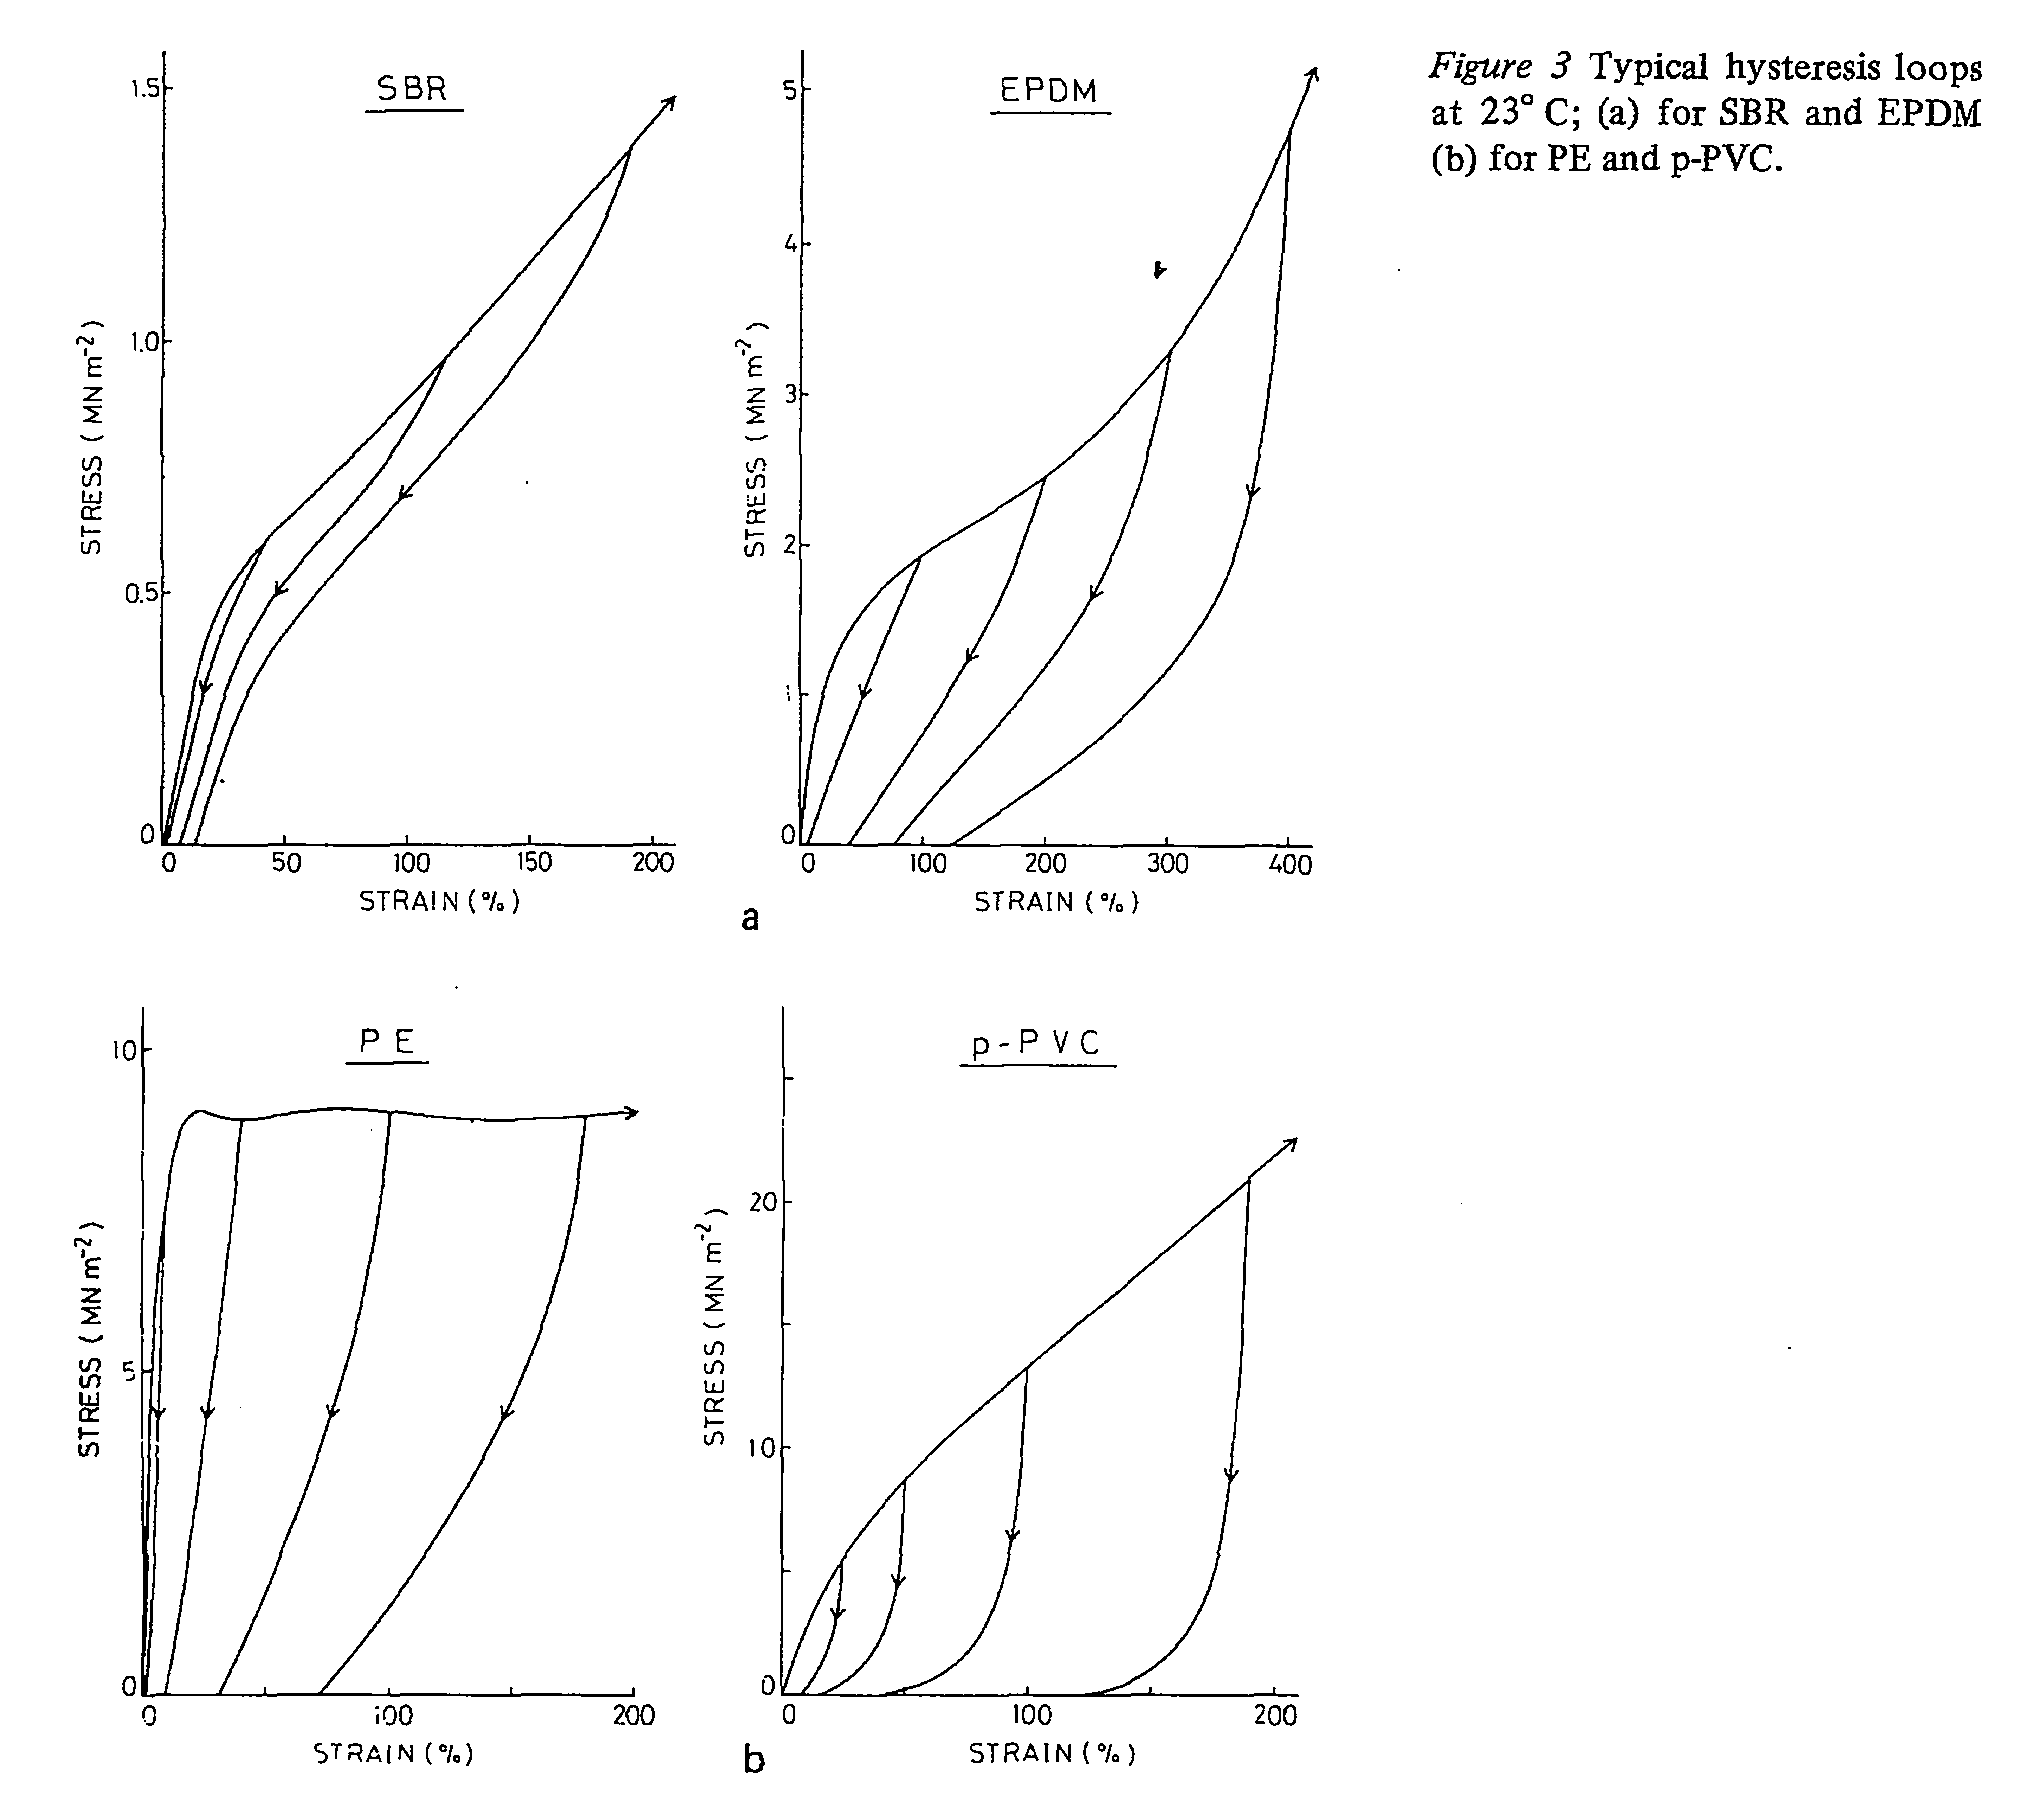
\includegraphics[width=\columnwidth]{fig/hysterisis_roop.png}
\column{.47\linewidth}

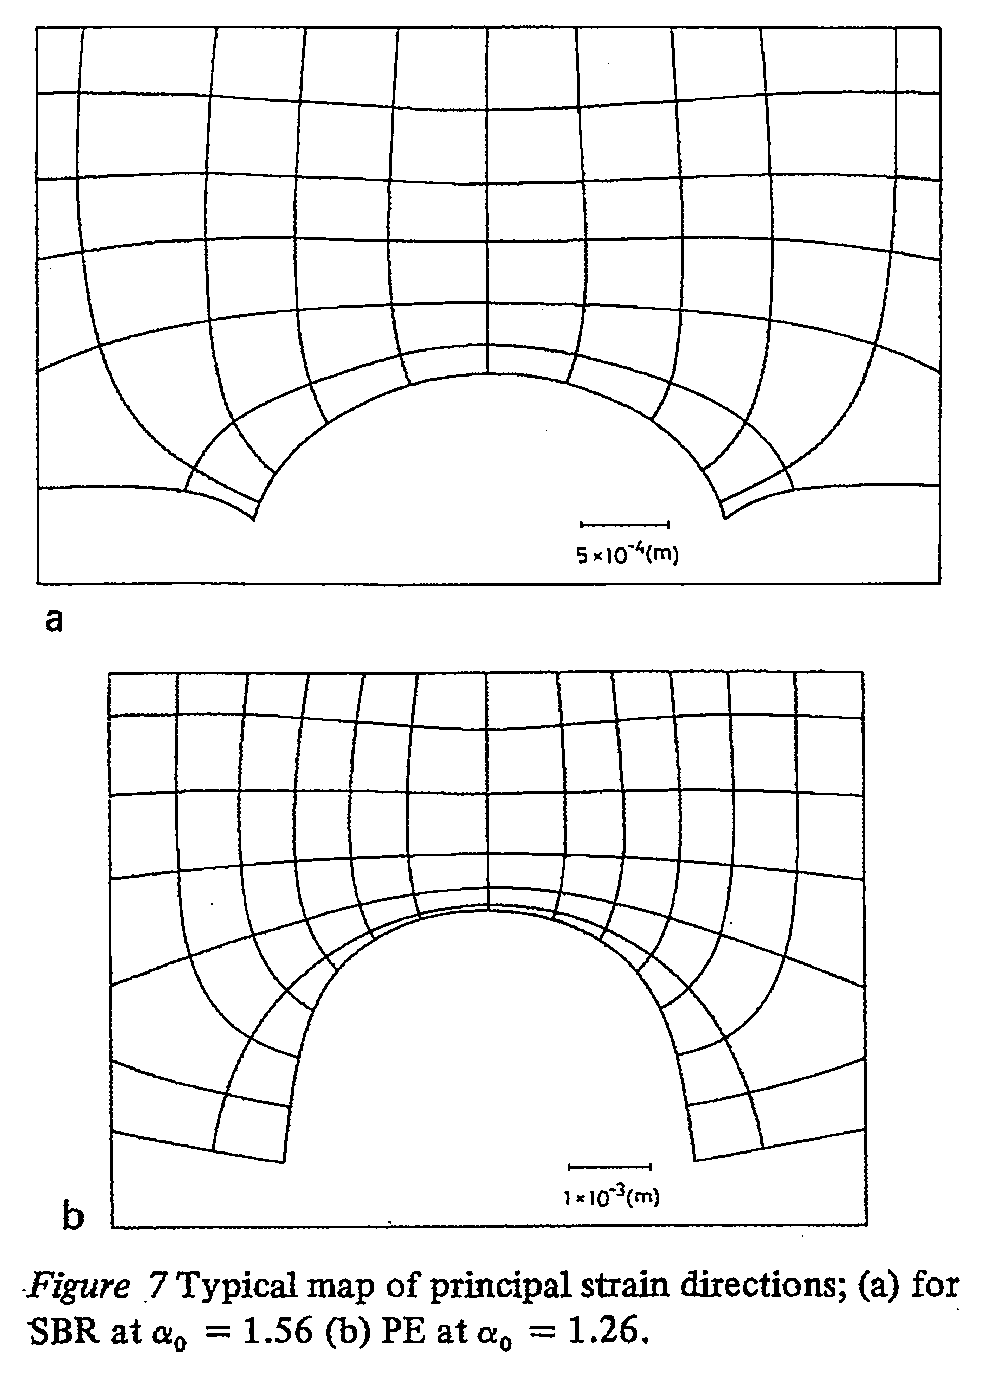
\includegraphics[width=\columnwidth]{fig/Typical_map.png}
\end{columns}

\end{frame}

%%%%%%%%%%%%%%%%%%%%%
\subsection{他の理論}
\begin{frame}
%[shrink squeeze]
%[allowframebreaks]
\frametitle{DNゲルについての理論}

``A local damage model for anomalous high toughness of double-network gels''\\
Tanaka, Y., Europhysics Letters, 78(5): 56005, 2007

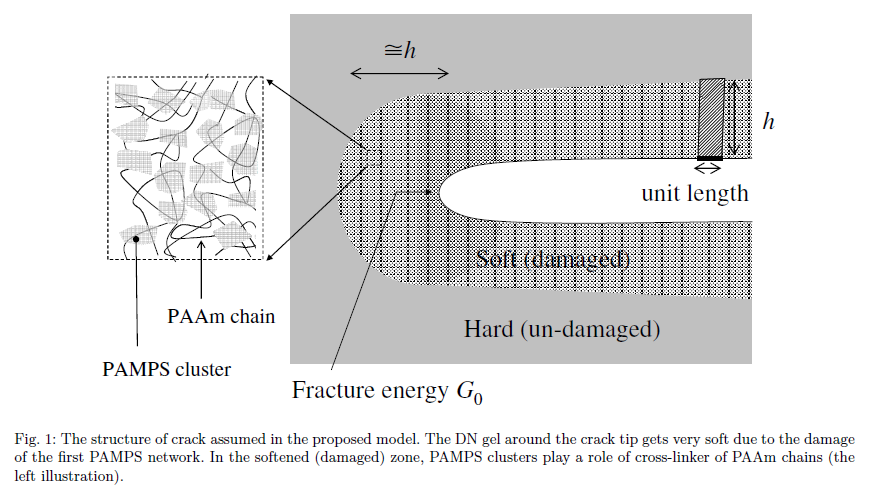
\includegraphics[width=\textwidth]{fig/tanaka.png}
\end{frame}

\end{document}
